
\scsubsection{Введение в язык графического представления баз знаний ostis-систем}
\label{intro_scg}

\begin{SCn}

\scnsectionheader{\currentname}

\scnstartsubstruct

\scnsegmentheader{Первый сегмент Введения в язык графического представления баз знаний ostis-систем}

\scnstartsubstruct

\scnheader{Введение в язык графического представления баз знаний ostis-систем}
\scnidtf{Введение в SCg-код}
\scnreltovector{конкатенация сегментов}{Первый сегмент Введения в SCg-код;Описание Ядра SCg-кода;Описание Первого расширения Ядра SCg-кода;Описание Второго расширения Ядра SCg-кода;Описание Третьего расширения Ядра SCg-кода;Описание Четвертого расширения Ядра SCg-кода;Описание Пятого расширения Ядра SCg-кода;Описание Шестого расширения Ядра SCg-кода;Описание Седьмого расширения Ядра SCg-кода;Последний сегмент Введения в SCg-код}

\scnheader{следует отличать*}
\scnhaselement{\scnset{\textit{SCg-код}; \textit{Введение в SCg-код}}}
\scnhaselement{\scnset{\textit{Ядро SCg-кода}; \textit{Описание Ядра SCg-кода}}}
\scnhaselement{\scnset{\textit{Первое расширение Ядра SCg-кода}; \textit{Описание Первого расширения Ядра SCg-кода}}}

\scnsourcecomment{То есть следует отличать саму описываемую сущность и текст, являющийся описанием этой сущности}

\scnheader{SCg-код}
\scnidtf{Semantic Code graphical}
\scnidtf{Язык визуального (графического) представления баз знаний ostis-систем}
\scnexplanation{SCg-код представляет собой способ визуализации sc-текстов (sc-конструкций) в виде рисунков этих конструкций. Подчеркнем, что абстрактная графовая структура и её рисунок (графическое изображение) -- это не одно и тоже даже, они изоморфны друг другу. SCg-код рассматривается нами как \textit{объединение*} нескольких его подъязыков, в число которых входит Ядро SCg-кода, обеспечивающее изоморфное графическое изображение любого sc-текста, а также несколько направлений расширения этого ядра, обеспечивающих повышение компактности и и читабельности текстов SCg-кода (sc.g-текстов, sc.g-конструкций).}

\scnendstruct

\scnsegmentheader{Описание Ядра SCg-кода}

\scnstartsubstruct

\bigskip
\scnfilelong{Алфавиту SC-кода взаимно однозначно соответствует алфавит \textit{Ядра SCg-кода} (алфавит sc.g-элементов, графически изображающих sc-элементы). Все sc-узлы, не являющиеся знаками файлов в тексте (конструкции) \textit{Ядра SCg-кода} изображаются в виде небольших чёрных кругов одинакового радиуса, который обозначим через $r$, и точная величина которого зависит от масштаба отображения sc.g-конструкции. Каждое \uline{sc-ребро} в \textit{Ядре SCg-кода} изображается в виде линии произвольной формы не имеющий самопересечений и имеющей толщину, равную примерно $r/8$.

Каждая \uline{sc-дуга} в \textit{Ядре SCg-кода} изображается в виде линии произвольной формы, не имеющей самопересечений, имеющей толщину равную $r/8$ и имеющей изображение стрелочки на одном из концов этой линии. 

Каждая входящая в sc-конструкцию \uline{базовая sc-дуга} в \textit{Ядре SCg-кода} изображается в виде линии произвольной формы, не имеющий самопересечений, имеющий толщину $r/4$, и имеющей изображение стрелочки на одном из ее концов. 

Каждый входящий в sc-конструкцию \uline{sc-узел}, имеющий содержимое, в \textit{Ядре SCg-кода} изображается в виде прямоугольника произвольного размера с толщиной линии $r/6$. Внутри этого прямоугольника отображается файл, обозначаемый изображаемым sc-узлом. Если нет необходимости изображать в тексте сам файл, обозначаемый sc-узлом, имеющим содержимое, то такой sc-узел в Sc.g-тексте изображается в виде прямоугольника со сторонами $2r$ по вертикали и $4r$ по горизонтали.

Представим таблицу соответствия между \textit{Алфавитом SC-кода} (Алфавитом абстрактных элементов sc-конструкций) и \textit{Алфавитом Ядра SCg-кода} (Алфавитом графических примитивов, составляющих конструкции Ядра SCg-кода и являющихся изображениями sc-элементов).}

\scnheader{Таблица. Алфавит Ядра SCg-кода}
\scneqfile{\\
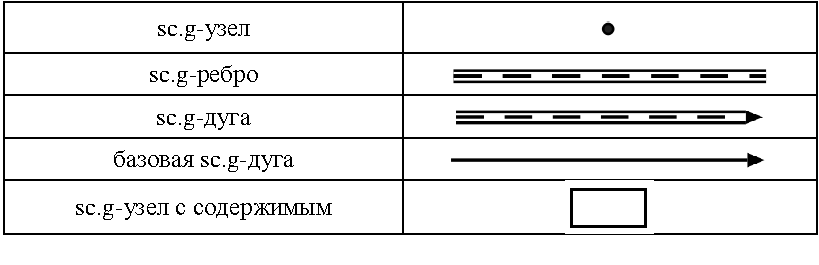
\includegraphics{figures/intro/SCg-core-alphabet.pdf}\\
}

\scnheader{Описание Ядра SCg-кода}
\scnseminclusion{Трудно сразу поверить, что на основе такого простого алфавита можно построить удобный и \uline{универсальный} графовый язык. В рамках \textit{Описания Технологии OSTIS} мы постараемся Вас в этом убедить. Кроме того, нас не должна настораживать простота алфавита, поскольку человечество имеет большой опыт кодирования, хранения в памяти и передачи по каналам связи самых различных информационных ресурсов, используя алфавит, состоящий только из двух классов элементов -- единиц и нулей. 

Мы ведем речь о принципиально ином (графовом) способе кодирования информации в компьютерных системах, но стараемся при этом свести это кодирование к достаточно простому алфавиту хотя бы для того, чтобы искусственно не усложнять проблему создания нового поколения компьютеров, основанных на указанном способе кодирования информации. 

Расширения \textit{Ядра SCg-кода} рассмотрим как направления перехода от текстов \textit{Ядра SCg-кода} к более компактным текстам. Но, поскольку это приводит к усложнению \textit{Синтаксиса SCg-кода} и, в первую очередь, к расширению \textit{Алфавита SCg-кода}, делать такие расширения необходимо обоснованно с учетом частоты встречаемости в рамках \textit{баз знаний ostis-систем} соответствующих фрагментов.}

\scnendstruct

\scnsegmentheader{Описание Первого расширения Ядра SCg-кода}

\scnstartsubstruct

\bigskip
\scnfilelong{Первое расширения Ядра SCg-кода -- это уточнение типологии константных постоянных сущностей и расширение \textit{Алфавита Ядра SCg-кода}, позволяющее типологию \textit{константных постоянных сущностей} привести в соответствие с синтаксической типологией вводимых элементов \textit{Алфавита SCg-кода}. 

Понятие константы противопоставляется понятию переменной. Константа -- это знак конкретной фиксированный сущности, которая в текущий момент не обязательно должна быть детально изучена. Переменная -- это обозначение некоторой абстрактной произвольной сущности, которая может принимать ("пробегать") \uline{значения} из некоторого множества сущностей. 

Понятие постоянной сущности противопоставляется понятию временной сущности. \textit{Постоянная сущность} -- сущность, существующая \uline{всегда}. \textit{Временная сущность} -- сущность, существующая в течение некоторого отрезка времени. 

Рассмотрим подробнее sc.g-элементы, знаки \textit{константных постоянных сущностей} различного вида. Графическим признаком \textit{константных постоянных sc-узлов} в конструкциях SCg-кода является их изображение в виде \uline{окружностей} радиуса $2r$. Какое изображение является более компактной записью факта принадлежности заданного sc-узла (назовем его $\bm{v_i}$) классу sc-констант и классу обозначений постоянных сущностей. Запись этого факта в \textit{Ядре SCg-кода} потребует (1) явного изображения sc-узла, обозначающего класс всевозможных константных sc-элементов (класс \textit{sc-констант}), (2) явного изображения базовой sc-дуги, соединяющего изображение sc-узла, обозначающего класс sc-констант, с изображением заданного константного sc-узла, (3) явного изображение sc-узла, обозначающего класс всевозможных sc-элементов, обозначающих \textit{постоянные сущности}, (4) явного изображения базовой sc-дуги, соединяющего изображение sc-узла, обозначающего класс обозначений \textit{постоянных сущностей} с изображением рассматриваемого sc-узла $\bm{v_i}$ (\textit{Файл. Изображение спецификации sc.g-элемента средствами Ядра SCg-кода и Первого расширения Ядра SCg-кода}).

Общепринятая запись данного факта выглядит следующим образом:

"\textit{sc-константа} $\ni \bm{v_i}$; \textit{постоянная сущность} $\ni \bm{v_i};$"

\textit{Константные постоянные sc-ребра} в конструкциях SCg-кода изображаются в виде двойной линии, каждая из которых имеет толщину $r/4$, а расстояние между ними также равно $r/4$. 

\textit{Константные постоянные sc-дуги} изображаются в виде такой же двойной линии, но со стрелочкой. Все базовые sc-дуги, а также все sc-узлы, имеющие содержимое, по определению являются \textit{константными постоянными sc-элементами}. 

\textit{Константные sc.g-узлы}, изображаемые окружностями радиуса $2r$, обозначают \textit{константные постоянные сущности}, о которых мало что известно, но известно то, что они не являются парами (то есть множествами, \textit{мощность*} которых равна 2) и, следовательно, не могут быть изображёны в виде sc.g-дуг или sc.g-рёбер. Но, если при этом об обозначаемой \textit{константной постоянной сущности} ($\bm{v_i}$) известно, что она является классом сущностей, то текст *** можно заменить на более компактный ***. 

Аналогичным образом: 
\begin{scnitemize}
\item sc.g-текст *** означает, что некая сущность $\bm{v_i}$ является \textit{отношением}; 
\item sc.g-текст *** означает, что некая сущность $\bm{v_i}$ является \textit{ролевым отношением}; 
\item sc.g-текст *** означает, что некая сущность $\bm{v_i}$ является \textit{небинарной связкой}; 
\item sc.g-текст *** означает, что некая сущность $\bm{v_i}$ является \textit{структурой}; 
\item sc.g-текст *** означает, что некая сущность $\bm{v_i}$ является первичный сущностью (терминальный сущностью, которая не является множеством, а также файлом, хранимым в памяти ostis-системы); 
\item sc.g-текст *** означает, что некая сущность $\bm{v_i}$ является файлом, хранимым в памяти ostis-системы;
\item sc.g-текст *** означает, что некая сущность $\bm{v_i}$ является файлом, хранимым в памяти ostis-системы, а знак этого файла обозначает также множество всевозможных его вхождений в другие файлы. 
\end{scnitemize}

Важное место среди константных постоянных сущностей занимают \textit{константные постоянные пары принадлежности}, обозначаемое соответствующими \textit{sc.g-дугами}. Такие пары принадлежности и обозначающие их sc.g-дуги бывают позитивными, негативными и нечеткими. Константная постоянная позитивная sc.g-дуга принадлежности есть ничто иное, как базовая sc.g-дуга. Константная постоянная негативная sc.g-дуга принадлежности изображается в виде "толстой"\ сплошной непунктирной линии со стрелкой и со штриховыми черточками. Константная постоянная нечёткая sc.g-дуга принадлежности изображается в виде толстой сплошной непунктирной линии со стрелкой и со штриховыми точками.}

\scnheader{Файл. Изображение спецификации sc.g-элемента средствами Ядра SCg-кода и Первого расширения Ядра SCg-кода}
\scneqfile{\\
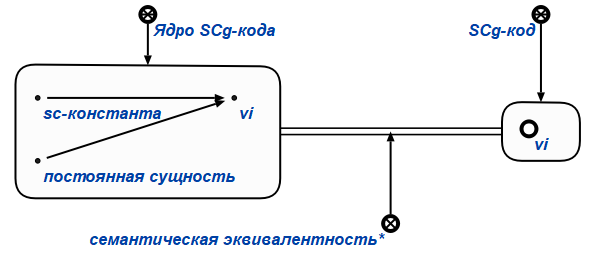
\includegraphics{figures/intro/scg1.png}\\
}
\scnendstruct

\scnsegmentheader{Описание Второго расширения Ядра SCg-кода}

\scnstartsubstruct

\bigskip
\scnfilelong{Второе расширение Ядра SCg-кода -- это расширение его алфавита путем введения дополнительных sc.g-элементов, обозначающих \textit{константные временные сущности} различного вида. Признаком sc.g-элементов, обозначающих \textit{константные временные сущности} являются точечные линии (линии, состоящие из точек, размер которых равен размеру изображаемой линии и которые близко расположены друг к другу на расстоянии, равном половине их размера), с помощью которых рисуются окружности при изображении sc-узлов, а также линии при изображении sc-коннекторов.

Результатом \textit{Второго расширения Ядра SCg-кода} является введение следующих видов sc.g-элементов (\textit{Таблица. sc.g-знаки константных временных сущностей}).
}

\scnheader{Таблица. sc.g-знаки константных временных сущностей}
\scneqfile{\\
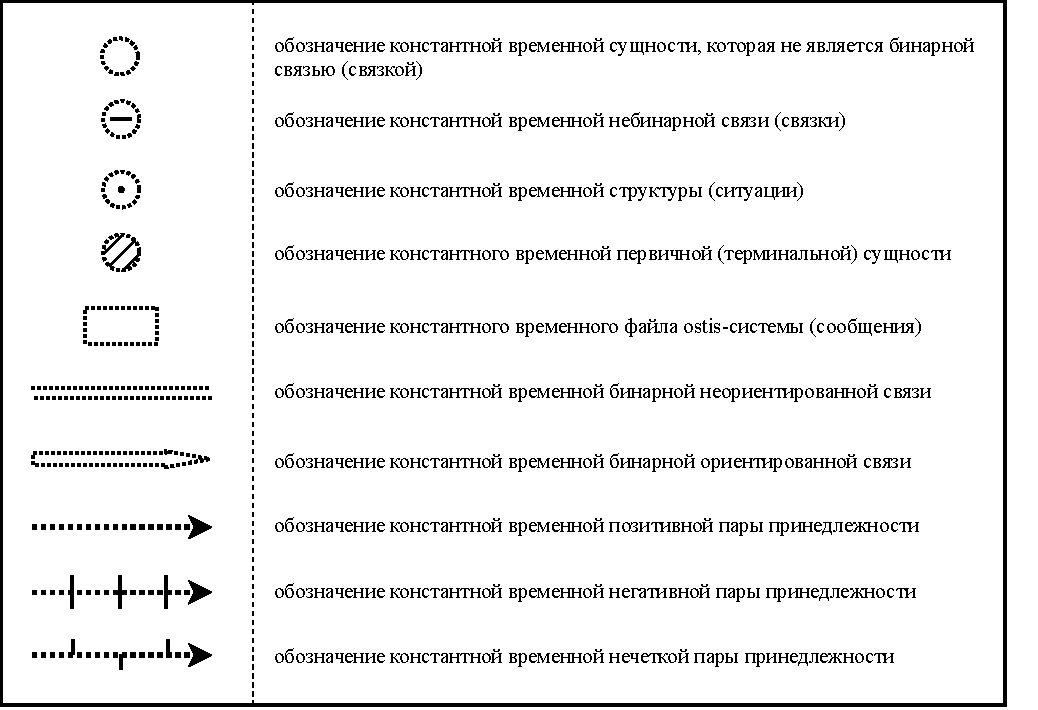
\includegraphics[width=1\linewidth]{figures/intro/SCg-temp-entities.pdf}\\
}

\scnendstruct

\scnsegmentheader{Описание Третьего расширения Ядра SCg-кода}

\scnstartsubstruct

\bigskip
\scnfilelong{Третья расширения ядра SCg-кода -- это расширение его алфавита путем введения дополнительных элементов, обозначающих \textit{переменные постоянные сущности} различного вида. Признаком sc.g-элементов, обозначающих сущности указанного класса, являются квадратики для изображения обозначений \textit{переменных постоянных сущностей}, не являющихся бинарными связями, а также пунктирные (в том числе и штрих-пунктирные) линии для изображения \textit{переменных постоянных бинарных связей}. 

Подчеркнем, что \textit{переменные постоянные сущности} могут отличаться друг от друга по характеру их \textit{области значений*}. Этими значениями в общем случае могут быть как \textit{константные постоянные сущности}, так и \textit{переменные постоянные сущности}. В любом случае, значение \textit{переменной сущности} является либо \textit{константной сущностью}, либо \textit{переменной сущностью}. Если каждое значение переменной является константой, то такую переменную будем называть \textit{переменной первого уровня}. Если каждое значение переменной является \textit{переменной первого уровня}, то такую переменную будем называть \textit{переменной второго уровня}. 

\textit{Переменная постоянная сущность первого уровня}, не являющаяся бинарной связью -- это переменная, каждым значением которой является \textit{константная постоянная сущность}, не являющаяся бинарной связью. Такая переменная изображается квадратиком, который ориентирован по вертикали и горизонтали. 

Указанная выше семантика такого изображения приписывается \uline{по умолчанию}. Это означает, что, если обозначаемая переменная имеет более сложную структуру области её значений, то эта область должна быть специфицирована явно. 

\textit{Переменная постоянная сущность второго уровня}, не являющаяся бинарной связью, изображается квадратиком, повернутым на 45$^\circ$.}

\scnheader{Таблица. sc.g-обозначения переменных постоянных сущностей}
\scneqfile{\\
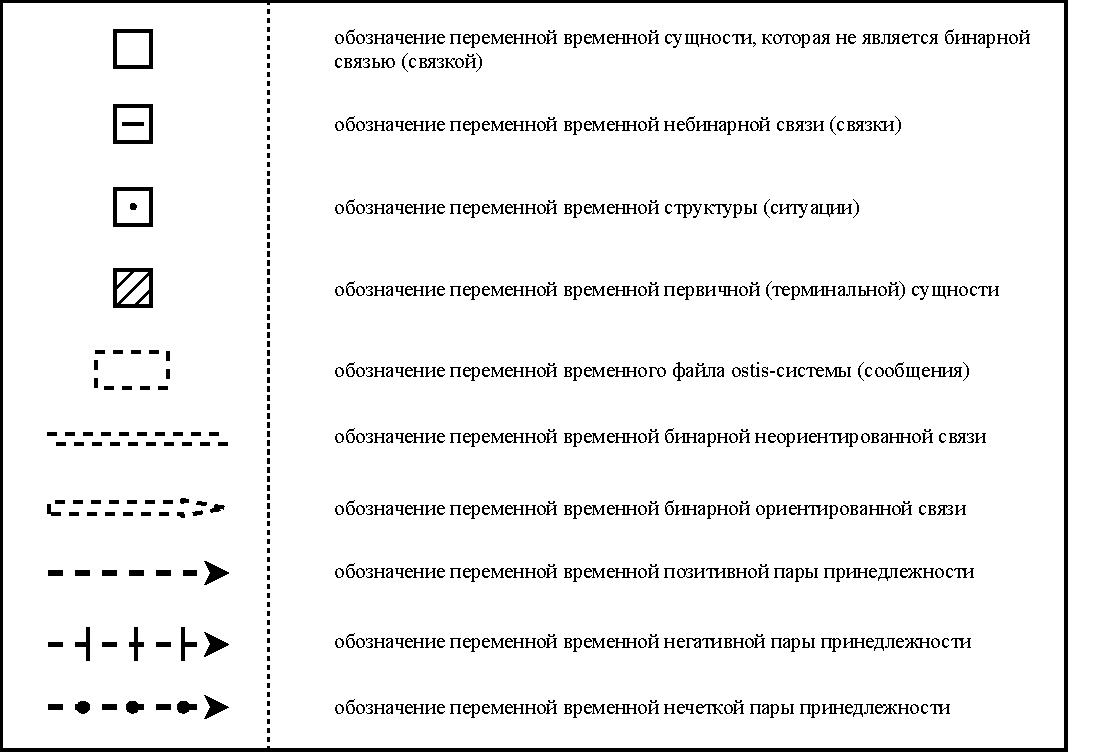
\includegraphics[width=1\linewidth]{figures/intro/SCg-var-entities.pdf}\\
}

\scnendstruct

\scnsegmentheader{Описание Четвертого расширения Ядра SCg-кода}

\scnstartsubstruct

\bigskip
\scnfilelong{Четвертое расширения Ядра SCg-кода -- это расширение его алфавита путем введения дополнительных sc.g-элементов, обозначающих \textit{переменные временные сущности} различного вида. Указанные дополнительные sc.g-элементы аналогичны тем, которые введены в рамках Второго расширения Ядра SCg-кода, и отличаются только тем, что в Четвёртом расширении Ядра SCg-кода речь идёт о переменных \uline{временных} сущностях, а во Втором расширении -- о переменных \uline{постоянных} сущностях.}

\scnendstruct

\scnsegmentheader{Описание Пятого расширения Ядра SCg-кода}

\scnstartsubstruct

\bigskip
\scnfilelong{Пятое расширение Ядра SCg-кода --  это приписывание некоторым sc.g-элементам \textit{основных внешних идентификаторов*} (чаще всего -- строковых идентификаторов, то есть имен) sc-элементов, изображаемых этими sc.g-элементами. Указанные идентификаторы являются уникальными для каждого идентифицируемого (именуемого) sc.g-элемента. Приписывание sc.g-элементам уникальных идентификаторов дает возможность в рамках одного sc.g-текста дублировать (копировать) некоторые sc.g-узлы при условии, если \uline{всем} таким копиям будут приписаны соответствующие идентификаторы. Такое дублирование sc.g-узлов является дополнительным средствам \uline{наглядного} размещения sc.g-текстов. 

Приписывание sc.g-элементу соответствующего ему основного (уникального) \textit{внешнего идентификатора*} представляет собой сокращённый вариант изображения sc.g-текстов, в которых приписывание идентификаторов отсутствует. Приведем пример. Пусть имеется некий sc.g-элемент, которому соответствует \textit{основной внешний идентификатор*} "$\bm{e_i}$". Этот факт без переписывания указанного идентификатора указанному sc.g-элементу будет выглядеть следующим образом (\textit{Файл. Пример идентификации sc.g-элемента без использования средств Пятого расширения Ядра SCg-кода}). 

Здесь отношение, связывающее sc.g-элементы с файлами, содержащими их основные внешние идентификаторы, само имеет свой основной внешний идентификатор, который представляет собой строку символов, имеющую вид "основной внешний идентификатор*". Нетрудно заметить, что с помощью средства приписывания идентификаторов sc.g-элементам приведенная выше конструкция будет выглядеть тривиально: ***.}

\scnheader{Файл. Пример идентификации sc.g-элемента без использования средств Пятого расширения Ядра SCg-кода}
\scneqfile{\\
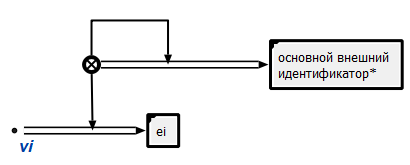
\includegraphics{figures/intro/scg2.png}\\
}

\scnendstruct

\scnsegmentheader{Описание Шестого расширения Ядра SCg-кода}

\scnstartsubstruct

\bigskip
\scnfilelong{\textbf{\textit{Шестое расширение Ядра SCg-кода}} -- это введение в SCg-код sc.g-контуров, sc.g-рамок и sc.g-шин как средств структуризации sc.g-текстов и повышения наглядности при их размещении. Подчеркнем, что и sc.g-контуры, и sc.g-шины, и sc.g-рамки являются специальными видами sc.g-элементов. При этом sc.g-контуры и sc.g-рамки являются sc.g-ограничителями (ограничителями SCg-кода).

Каждый sc.g-контур изображается (в 2D-модификации) в виде замкнутой ломаной линии, ограничивающей некоторый фрагмент sc.g-текста и обозначает множество всех \uline{sc-элементов}, sc.g-изображения которых оказались внутри этого контура.

Обозначение множества sc-элементов, изображаемое sc.g-контуром, может быть как константным, так и переменным. Соответственно этому линия, изображающая sc.g-контур может быть: 

\begin{scnitemize}
\item неточечной линией без пропусков,
\item точечной линией без пропусков,
\item неточечной пунктирной линией,
\item точечной пунктирной линией.
\end{scnitemize}

Семантическим эквивалентом sc.g-контуру является sc.g-узел, обозначающий sc-структуру. Использование sc.g-контура вместо указанного sc.g-узла исключает необходимость явно изображать SC-дуги принадлежности, выходящие из этого sc.g-узла. Это существенно повышает уровень наглядности sc.g-текста.

Если представленный внутри sc.g-контура текст не является sc.g-текстом, то считается, что что на самом деле внутренностью sc.g-контура является sc.g-текст, являющийся результатом переводя предоставленного текста в SCg-код.

Каждая sc.g-рамка является ограничителем изображения файла, обозначаемого этой sc.g-рамкой. Таким образом, sc.g-рамка может быть sc.g-ограничителем не только sc.g-текстов, но и любых других инородных для SCg-кода информационных конструкций, изображаемых на плоскости.

Семантическим эквивалентом sc.g-рамок являются sc.g-узлы следующего вида (\textit{Файл. Примеры SCg-рамок различного вида}).

Соответственно этому, sc.g-рамки всегда являются константными, хотя переменные, значениями которых являются sc.g-узлы, обозначающие файлы-ostis-систем, существуют, но  содержимого эти переменные иметь не могут.

Каждая sc.g-шина представляет собой замкнутую или незамкнутую линию, которая инцидентна только одному sc.g-элементу и семантически ему эквивалентна. Идея введения sc.g-шин заключается в увеличении «размеров» sc.g-элементов для расширения их области инцидентности. Особенно актуально это для sc.g-узлов, имеющих большое число инцидентных им sc.g-коннекторов.}

\scnheader{Файл. Примеры SCg-рамок различного вида}
\scneq{\scnfileshort{c.70}}

\scnendstruct

\scnsegmentheader{Описание Седьмого расширения Ядра SCg-кода}

\scnstartsubstruct

\bigskip
\scnfilelong{\textbf{\textit{Седьмое расширение Ядра SCg-кода}} -- это переход от 2D-изображений sc.g-текстов к 3D-изображениям.
Одним из вариантов трехмерного изображения sc.g-текстов является следующий:

\begin{scnitemize}
\item все sc.g-узлы изображаются, как и ранее, \uline{плоскими} графическими примитивами. При изменении точки просмотра они \uline{всегда} "поворачиваются"\ параллельно плоскости экрана, но их масштаб (размер на экране) при удалении от  точки просмотра \uline{уменьшается};
\item аналогичным "плоским"\ образом изображаются sc.g-рамки с их "внутренним"\ содержанием, а также внешние идентификаторы, приписываемые sc.g-элементам;
\item sc.g-коннекторы изображаются \uline{непересекающимися} линиями в трехмерном пространстве (заметим, что при изображении sc.g-текстов на плоскости пересечение sc.g-коннекторов часто снижает наглядность, "читательность"\ sc.g-текстов). Т.е. sc.g-коннекторы, которые на плоскости изображаются двойными линиями, в пространстве  цилиндрическими, "трубчатыми линиями"\ с находящейся внутри тонкой, но просвечивающейся осевой линией;
\item sc.g-контур в пространстве визуализируется несколькими (!) специального вида точками -- например там, где есть точки инцидентности sc.g-контура с \uline{внешними} sc.g-коннекторами. При этом sc.g-контур становится виден только по команде просмотра указываемого контура (указание контура – это указание одной из его точек инцидентности). По этой команде цветом выделяются все граничные точки контура (точки инцидентности) и все внутренние sc.g-элементы контура. Если просматривается  несколько контуров, то используется несколько цветов.
\end{scnitemize}

Вторым вариантом 3D-визуализации sc.g-текстов является размещение sc.g-текстов на параллельных плоскостях (слоях) с “прошивками”\ между этими слоями, соединяющими синонимичные sc.g-узлы, т.е. sc.g-узлы, имеющие одинаковые приписываемые им внешние идентификаторы. Такой вариант плоской, но многослойной визуализации sc.g-текстов дает возможность широко использовать те средства просмотра и редактирования sc.g-текстов, которые разработаны для плоской их визуализации.}

\scnendstruct

\scnsegmentheader{Последний сегмент Введения в SCg-код}

\scnstartsubstruct

\bigskip
\scnfilelong{Основная цель SCg-кода – иметь четкие синтаксические графические признаки изображения sc.g-элементов, позволяющие легко выделить и различать такие классы sc.g-элементов, как:

\begin{scnitemize}
\item sc.g-константы (знаки константных сущностей) и sc.g-переменные (изображения переменных, значениями которых являются соответсвующие sc.g-элементы);
\item sc.g-переменные, значениями которых являются константы, и sc.g-переменные, значениями которых являются переменные;
\item знаки постоянных (стабильных) сущностей и знаки временных (нестабильных, временно существующих, ситуативных) сущностей;
\item sc.g-коннекторы (знаки бинарных связей) и sc.g-элементы, не являющиеся sc.g-коннекторами;
\item неориентированные sc.g-коннекторы (sc.g-ребра) и ориентированные (sc.g-дуги);
\item sc.g-дуги принадлежности и sc.g-дуги, не являющиеся таковыми;
\item sc.g-дуги позитивной принадлежности, негативной принадлежности и нечеткой принадлежности.
\end{scnitemize}

Приведен перечень элементов Алфавита SCg-кода (см. Алфавит SCg-кода).
Этот перечень оформлен в виде sc.g-текста и представляет собой изображение примеров всех введенных видов sc.g-элементов (по одному примеру каждого вида). При этом, указанные примеры sc.g-элементов разбиты на пять групп (\textit{Текст SCg-кода. Алфавит SCg-элементов}). Первая группа (верхняя строка) включает в себя sc.g-элементы, для которых константность и постоянство обозначаемых ими сущностей требует дополнительного уточнения. Остальные четыре группы sc.g-элементов аналогичны друг другу и включают в себя соответственно:

\begin{scnitemize}
\item знаки \uline{константных постоянных} сущностей;
\item знаки \uline{константных временных} сущностей;
\item изображения переменных, значениями которых или значениями значений которых (в случае, если значениями переменных являются переменные) являются знаки константных \uline{постоянных} сущностей;
\item изображения переменных, значениями которых или значениями значений которых (в случае, если значениями переменных являются переменные) являются знаки константных \uline{временных} сущностей.
\end{scnitemize}

Особое место в Алфавите SCg-кода занимает графическое изображение SC-дуги принадлежности в виде сплошной непунктирной “толстой”\ линии со стрелкой и с размещенными на ней штрихованными точками и черточками.
Этот sc.g-элемент будем называть \textit{sc.g-дугой принадлежности}.
Данный sc.g-элемент используется тогда, когда нам необходимо изобразить SC-дугу, о которой известно, что она является SC-дугой принадлежности, но неизвестно о какой принадлежности идет речь -- о константной или переменной, о постоянной или временной, о позитивной, негативной или нечеткой.

Кроме sc.g-элементов, перечисленных в \textit{Текст SCg-кода. Алфавит SCg-кода}, в состав Алфавита SCg-кода входят также следующие sc.g-элементы:
\begin{scnitemize}
\item внешние идентификаторы sc.g-элементов, идентичные (приписываемые) сответствующим sc.g-элементам.
\item sc.g-контуры, каждый из которых является знаком некоторого sc-текста (структуры, состоящей из sc-элементов). Каждый такой sc-текст может быть:
\begin{scnitemizeii}
\item либо константной постоянной структурой (см. sc.g-элемент типа ***);
\item либо константной постоянной структурой (ситуацией) -- см. sc.g-элемент типа ***;
\item либо переменной структурой, значениями которой являются \uline{постоянные} структуры изоморфной  конфигурации (см. sc.g-элемент ***);
\item либо переменной структурой, значениями которой являются \uline{временные} структуры (ситуации) изоморфной  конфигурации (см. sc.g-элемент ***);
\end{scnitemizeii}

\item \textit{sc.g-рамки}, являющиеся ограничителями изображения различных файлов, хранимых в памяти ostis-системы (см. sc.g-элемент ***);
\item sc.g-шины, являющиеся обозначениями тех же сущностей, что и инцидентные им sc.g-элементы.
\end{scnitemize}

Заметим также, что, кроме всех перечисленных элементов Алфавита SCg-кода, каждый из которых имеет вполне определенную денотационную  семантику, для формализации синтаксиса SCg-кода необходимо ввести целый ряд более "мелких"\ синтаксических объектов, например:
\begin{scnitemize}
\item точек инцидентности sc.g-коннекторов с sc.g-узлами, с другими sc.g-коннекторами, с sc.g-контурами, с sc.g-рамками;
\item точек инцидентности sc.g-шин;
\item точек излома линейных sc.g-элементов (sc.g-коннекторов, sc.g-контуров, sc.g-рамок, sc.g-шин).
\end{scnitemize}
}

\scnheader{Текст SCg-кода. Алфавит SCg-кода}
\scneqfile{\\
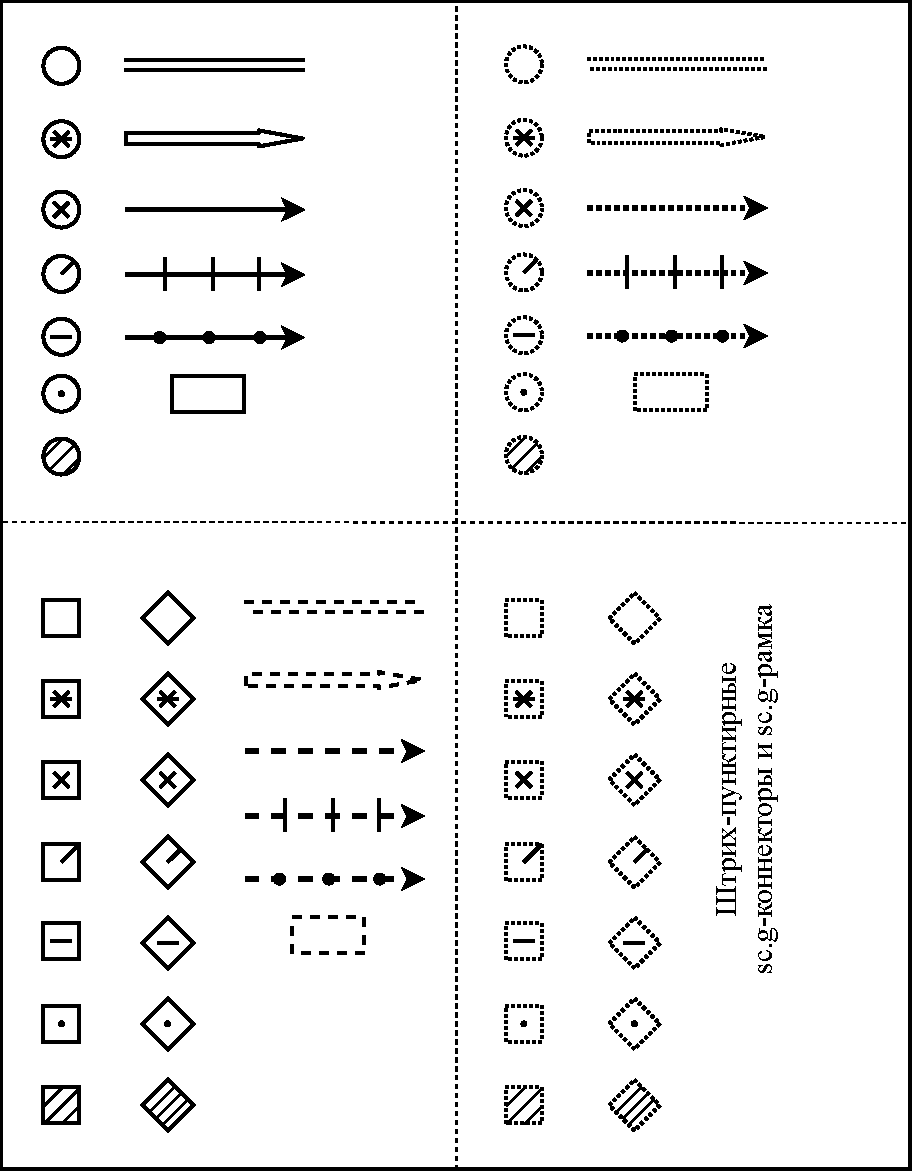
\includegraphics[width=1\linewidth]{figures/intro/SCg-full.pdf}\\
}


\scnendstruct

%End
\scnendstruct

\end{SCn}
